\documentclass[11pt]{article}

\usepackage{cmap}
\usepackage[utf8]{inputenc}
\usepackage[T1]{fontenc}
\usepackage[spanish,es-noindentfirst]{babel}
\usepackage[margin=2.5cm]{geometry}
\usepackage{booktabs}
\usepackage{graphicx}
\usepackage{hyperref}
\usepackage{caption}
\usepackage{amsmath}
\usepackage{float}

\hypersetup{colorlinks=true, linkcolor=blue, citecolor=blue, urlcolor=blue}

\title{Accesibilidad a salud de emergencia en Per\'u: tiempos de viaje\\
por carretera hacia establecimientos resolutivos\\
\large en Piura, Cusco y Loreto}
\author{HW\_02\_202602 --- Data Science}
\date{Septiembre 2026}

\begin{document}

\maketitle

\begin{abstract}
\noindent
Se construy\'o un pipeline reproducible que estima, para 10{,}801 puntos de
demanda (4.66 millones de habitantes) en Piura, Cusco y Loreto, el tiempo de
viaje por carretera hacia el establecimiento de salud resolutivo
(categor\'ia II-1 o superior, activo) m\'as cercano, usando OSRM sobre el
extracto de OpenStreetMap de Per\'u. El hallazgo central es la brecha entre
regiones: mientras el 78\% de la poblaci\'on conjunta llega en menos de 60
minutos, en Loreto el 43.9\% de los puntos de demanda no tiene ning\'un
tiempo de acceso vial confiable ---la red mapeada en OpenStreetMap es
pr\'acticamente inexistente fuera de Iquitos--- y 162 puntos (9\%) carecen
de cualquier ruta v\'alida. El coeficiente de Gini ponderado por poblaci\'on
del tiempo de acceso es 0.722 en conjunto (0.713 Piura, 0.650 Cusco, 0.696
Loreto). El distrito con peor acceso confiable es Manseriche (Loreto, 692
minutos ponderados). Se documentan seis reglas de validaci\'on de datos, una
sustituci\'on de fuente forzada por la falta de un endpoint estable en
MINEDU/SIGMED, y las limitaciones metodol\'ogicas del ruteo veh\'icular en
la Amazon\'ia.
\end{abstract}

\section{Introducci\'on y planteamiento del problema}

En emergencias m\'edicas, la ``hora dorada'' es la ventana en la que un
trauma severo o una emergencia obst\'etrica debe llegar a un establecimiento
capaz de resolverla. En Per\'u, un puesto de salud de categor\'ia I-1 puede
estabilizar a un paciente pero no puede operar ni atender una ces\'area; solo
los establecimientos de categor\'ia II-1 en adelante tienen esa capacidad
resolutiva. La pregunta que este trabajo busca responder es: \emph{\textbf{
¿cu\'anto tarda realmente, por carretera, la poblaci\'on de una regi\'on dada
en llegar a un establecimiento de salud con capacidad resolutiva, y d\'onde
est\'an las peores brechas?}}

La palabra ``realmente'' es la dif\'icil. Una l\'inea recta en un mapa no es
una carretera. Un establecimiento que figura en el registro puede estar
cerrado. Una coordenada del registro puede estar en el hemisferio
equivocado. Este reporte documenta c\'omo se trat\'o cada uno de esos
problemas y qu\'e tan bien --- o tan mal --- se pudieron resolver con datos
abiertos peruanos.

Por alcance, el an\'alisis no es nacional. Se seleccionaron tres
departamentos que representan las tres macrorregiones de Per\'u: \textbf{
Piura} (costa), \textbf{Cusco} (andino) y \textbf{Loreto} (amaz\'onico). El
contraste geogr\'afico es, deliberadamente, el punto anal\'itico del
ejercicio: como se ver\'a, un departamento costero y uno amaz\'onico no se
comportan igual frente al mismo m\'etodo de an\'alisis, y esa diferencia es
en s\'i misma uno de los hallazgos.

\section{Fuentes de datos}

\begin{itemize}
  \item \textbf{RENIPRESS / SUSALUD} (oferta --- establecimientos de
  salud). CSV mensual descargado de datosabiertos.gob.pe el 4 de
  septiembre de 2026 (edici\'on de agosto 2026, 36{,}004 registros a nivel
  nacional). Licencia Open Data Commons Attribution.
  \item \textbf{Centros poblados dispersos} (demanda rural, con
  poblaci\'on). Servicio ArcGIS REST del geoportal IDEP (Infraestructura de
  Datos Espaciales del Per\'u), datos de fuente INEI (Censos Nacionales
  2017). Descargado el 4 de septiembre de 2026. \textbf{Esta es una
  sustituci\'on documentada}: el enunciado original pide el ``spatial
  download'' de MINEDU/SIGMED, pero esa herramienta result\'o ser una
  aplicaci\'on ASP.NET WebForms interactiva (postbacks y ViewState) sin
  URL de descarga estable ni re-ejecutable program\'aticamente. El
  servicio del IDEP s\'i lo es.
  \item \textbf{Capitales distritales} y \textbf{poblaci\'on distrital
  proyectada 2018--2026} (INEI, xlsx oficial de gob.pe). Usadas para
  construir un punto de demanda urbano sint\'etico por distrito, ya que
  ninguna capa p\'ublica del geoportal cubre la poblaci\'on urbana
  concentrada como puntos individuales.
  \item \textbf{L\'imites administrativos}. Common Operational Dataset
  (COD-AB) de Per\'u, publicado por OCHA/HDX, fuente original Instituto
  Geogr\'afico Nacional (IGN). Vigente al 2020-07-14. Tres niveles:
  departamento (25), provincia (196), distrito (1{,}873).
  \item \textbf{OpenStreetMap}, extracto de Per\'u (Geofabrik,
  \texttt{peru-260903.osm.pbf}, 245\,MB), descargado el 3 de septiembre de
  2026.
\end{itemize}

Limitaciones conocidas de cada fuente se retoman en la Secci\'on
\ref{sec:limitaciones}.

\section{Metodolog\'ia}

\subsection{Definici\'on de establecimiento resolutivo}

Un establecimiento cuenta como resolutivo si y solo si su estado operativo
es \texttt{ACTIVO} y su categor\'ia normalizada es II-1, II-2, II-E, III-1,
III-2 o III-E. El campo \texttt{CATEGORIA} de RENIPRESS usa el valor
literal \texttt{"0"} para establecimientos a los que no aplica la escala
I-1..III-E (servicios m\'edicos de apoyo, establecimientos sin
internamiento): 1{,}202 de los 4{,}512 registros de los tres departamentos
(26.6\%) caen en este caso y se normalizan a \texttt{SIN\_CATEGORIA}. El
campo \texttt{ESTADO} result\'o ser, al inspeccionarlo, un vocabulario
controlado limpio (7 valores \'unicos, sin variantes tipogr\'aficas):
\texttt{ACTIVO} y seis variantes de baja o cierre temporal/definitivo; solo
\texttt{ACTIVO} cuenta como operativo.

\subsection{Validaci\'on de datos (Fase 1b)}

Se aplicaron seis reglas de calidad de datos sobre los 4{,}512
establecimientos de los tres departamentos (Tabla~\ref{tab:validacion}).
Ning\'un registro se descarta silenciosamente: cada regla agrega una
columna de bandera al dataset procesado
(\texttt{data/processed/renipress\_validado.parquet}), y la decisi\'on
tomada queda documentada. Dos hallazgos merecen menci\'on:

\begin{itemize}
  \item \textbf{29\% de los registros no tiene coordenadas utilizables}
  (nulas o efectivamente cero, $|\text{valor}| < 0.001\,^{\circ}$). Los
  campos de coordenadas de RENIPRESS se llaman \texttt{NORTE}/\texttt{ESTE}
  ---nombres que sugieren UTM--- pero contienen en realidad grados
  decimales WGS84 (\texttt{NORTE}=latitud, \texttt{ESTE}=longitud),
  verificado contra el rango geogr\'afico de Per\'u.
  \item \textbf{15.6\% de los registros geocodificados (499 de 3{,}203
  verificables) caen fuera del pol\'igono del distrito que declara su
  propio UBIGEO.} Se verific\'o que esto no es un error del pipeline: 498
  de esos 499 caen dentro de un distrito \emph{real} distinto al
  declarado, mayormente distritos contiguos dentro de la misma ciudad
  (Cusco/San Sebasti\'an/Wanchaq, Piura/Castilla/Veintis\'eis de Octubre),
  consistente con imprecisi\'on de geocodificaci\'on en zonas urbanas
  densas donde el l\'imite distrital cruza la propia manzana.
\end{itemize}

\begin{table}
\caption{Reglas de validaci\'on aplicadas a RENIPRESS (Fase 1b).}
\label{tab:validacion}
\begin{tabular}{lrl}
\toprule
Regla & N marcados & Acción \\
\midrule
1 coords missing or zero & 1309 & Se mantienen en el dataset (columna coords\_utilizables=False); se excl... \\
2 coords outside bbox & 0 & Se mantienen en el dataset (columna coords\_utilizables=False); se excl... \\
3 coords swapped & 0 & Ninguna encontrada en estos 3 departamentos; de existir, la correccion... \\
4 outside declared district & 499 & Se mantienen en el dataset con la bandera activada; no se excluyen aut... \\
5 duplicate cod ipress & 0 & Ninguno encontrado. \\
6 encoding issues & 0 & Ninguno encontrado en RENIPRESS para estos 3 departamentos (si apareci... \\
\bottomrule
\end{tabular}
\end{table}


\subsection{Ruteo (Fase 2)}

Se levant\'o un servidor OSRM local (Docker, algoritmo MLD, perfil
\texttt{car}) sobre el grafo construido a partir del extracto de Per\'u.
Para cada departamento se calcul\'o la matriz completa origen (demanda)
\'x destino (oferta resolutiva) v\'ia el endpoint \texttt{/table}, en
lotes de 150 puntos de demanda para no exceder l\'imites de URL. La
demanda combina centros poblados dispersos (rurales, con poblaci\'on
censal real) y un punto de demanda urbano sint\'etico por distrito
(poblaci\'on urbana estimada = poblaci\'on total proyectada INEI 2026
menos poblaci\'on dispersa, ubicado en la ``Capital de Distrito'' del
gazetteer nacional del IGN, o en el centroide del pol\'igono distrital
cuando el distrito no tiene un punto de capital en esa capa: 48 de 230
distritos). En total, 10{,}801 puntos de demanda y 72 establecimientos
resolutivos con coordenadas utilizables (32 Piura, 26 Cusco, 14 Loreto).

Cada consulta a OSRM devuelve, adem\'as de duraci\'on y distancia por red,
la distancia de \emph{snapping} (qu\'e tan lejos qued\'o el punto original
del nodo de red m\'as cercano usado para rutear). Un punto se marca
\texttt{snap\_confiable} cuando esa distancia es $\leq 5$\,km en ambos
extremos del par. Adem\'as, se descubri\'o en el an\'alisis que un snap
``confiable'' puede seguir produciendo una duraci\'on sin sentido si la
v\'ia mapeada es una trocha que el perfil de auto trata como casi
intransitable: el caso verificado fue el distrito de Ram\'on Castilla
(Loreto), con una ruta de 409\,km resuelta en 4{,}906 minutos, es decir 5.0
km/h de velocidad promedio. Se agreg\'o entonces un segundo chequeo
---velocidad promedio impl\'icita $\geq 8$\,km/h--- y solo los puntos que
pasan ambos chequeos se clasifican \texttt{confiable}; el resto queda como
\texttt{no\_confiable} (hay ruta, pero no es fiable) o \texttt{sin\_ruta}
(no existe ninguna ruta a ninguna facility).

\subsection{Construcci\'on de m\'etricas (Fase 3)}

Todas las m\'etricas se calculan \'unicamente sobre puntos
\texttt{confiable}, para no contaminar los promedios con duraciones sin
sentido; los puntos \texttt{no\_confiable} y \texttt{sin\_ruta} se
reportan siempre por separado, nunca se descartan del dataset. Las
m\'etricas construidas son: tiempo de acceso individual $t_{min}(i)$;
bandas de cobertura poblacional a 30/60/120 minutos y m\'as de 120;
tiempo de acceso promedio ponderado por poblaci\'on a nivel
distrito/provincia/departamento; lista de distritos cr\'iticos (peor
acceso ponderado, con un m\'inimo de 50 habitantes para evitar que un
distrito min\'usculo con mala suerte de ruteo domine el ranking);
coeficiente de Gini y curva de Lorenz del tiempo de acceso (los puntos
\texttt{sin\_ruta} se topean a 240 minutos para el c\'alculo de Gini, en
vez de excluirse, porque excluir a los peor servidos subestimar\'ia la
desigualdad real); contraste urbano/rural; y un cruce con una segunda
dimensi\'on (tama\~no de poblaci\'on del centro poblado, como proxy de
ruralidad, ante la ausencia de datos de pobreza o altitud en este
proyecto).

\section{Resultados}

\subsection{Cobertura y acceso ponderado}

La Figura~\ref{fig:coverage} muestra la distribuci\'on de la poblaci\'on
por banda de tiempo de acceso en cada departamento. Piura y Cusco tienen
perfiles similares, dominados por la banda de 30 minutos o menos (72.1\%
y 61.4\% de la poblaci\'on respectivamente). Loreto es cualitativamente
distinto: 41.7\% de su poblaci\'on cae en la categor\'ia ``sin dato
confiable'' y 2.2\% adicional en ``sin ruta vial'' (43.9\% en conjunto).

\begin{figure}[H]
  \centering
  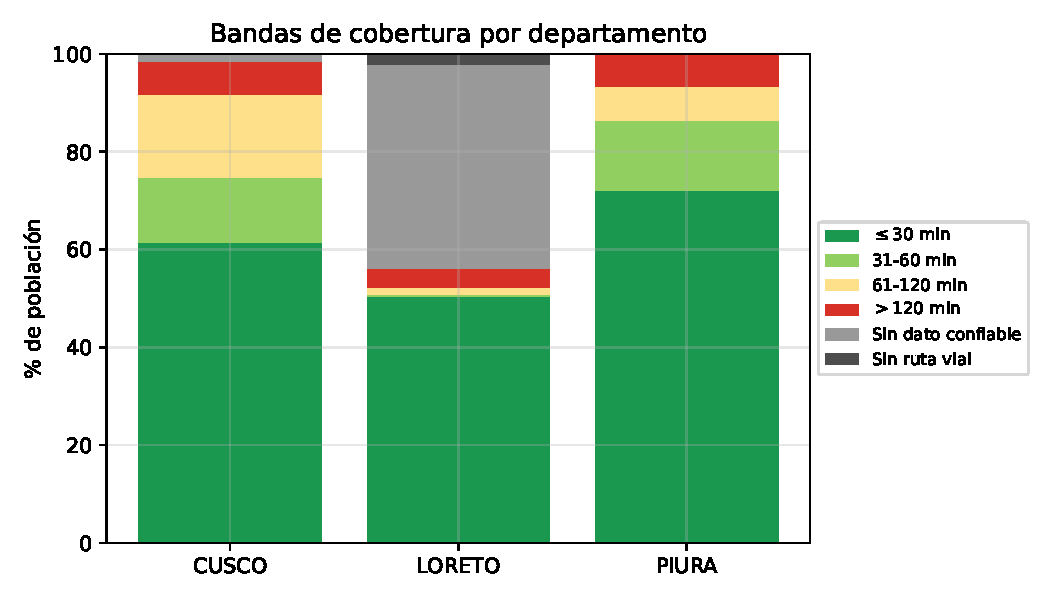
\includegraphics[width=0.85\textwidth]{figures/coverage_bands.pdf}
  \caption{Bandas de cobertura poblacional por departamento.}
  \label{fig:coverage}
\end{figure}

\begin{table}
\caption{Resumen de acceso por departamento.}
\label{tab:access_departamento}
\begin{tabular}{lllll}
\toprule
Departamento & Población & T. acceso ponderado (min) & Gini & \% sin dato confiable \\
\midrule
Cusco & 1,396,496 & 33.6 & 0.650 & 1.6\% \\
Piura & 2,195,231 & 26.3 & 0.713 & 0.0\% \\
Loreto & 1,066,046 & 22.7 & 0.696 & 43.9\% \\
\bottomrule
\end{tabular}
\end{table}


La Tabla~\ref{tab:access_departamento} resume el acceso ponderado por
departamento. El tiempo ponderado de Loreto (22.7 min) es enga\~nosamente
bajo: al calcularse solo sobre el 56\% de su poblaci\'on con dato
confiable ---dominado por Iquitos, donde el acceso es genuinamente
r\'apido--- no refleja la situaci\'on del resto del departamento. El
Gini ponderado por poblaci\'on (Figura~\ref{fig:lorenz}) es 0.722 en
conjunto. Entre Piura y Cusco --- los dos departamentos con una muestra
confiable representativa, a diferencia de Loreto --- Piura tiene mejor
tiempo promedio (26.3 min vs. 33.6 min) pero tambi\'en mayor Gini (0.713
vs. 0.650): indicio de una brecha interna marcada entre su franja
costera bien conectada y su sierra (Huancabamba), mientras que el acceso
en Cusco, aunque en promedio algo m\'as lento, est\'a algo m\'as
homog\'eneamente distribuido.

\begin{figure}[H]
  \centering
  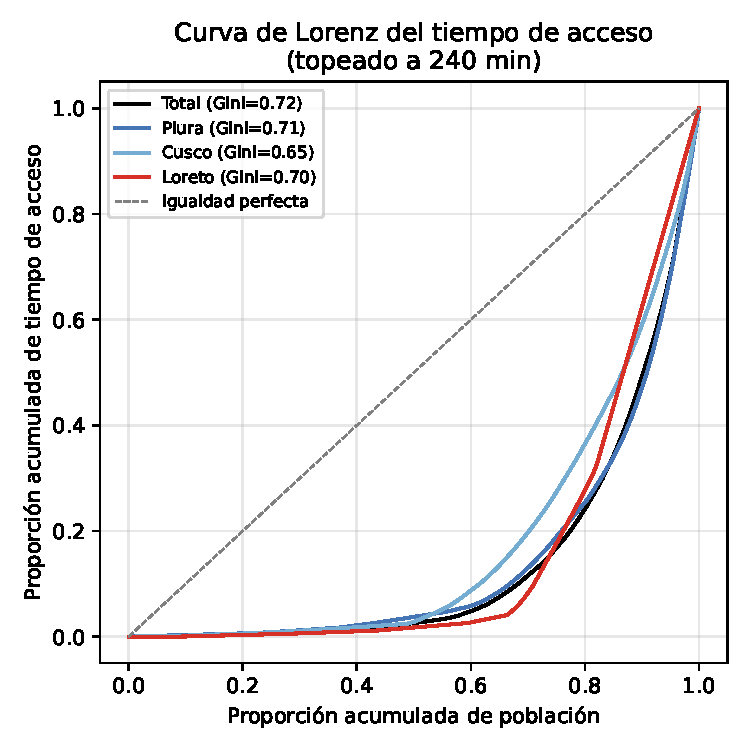
\includegraphics[width=0.6\textwidth]{figures/lorenz.pdf}
  \caption{Curva de Lorenz del tiempo de acceso ponderado por
  poblaci\'on.}
  \label{fig:lorenz}
\end{figure}

\subsection{Distritos cr\'iticos}

\begin{table}
\caption{Los 10 distritos con peor acceso ponderado por poblaci\'on.}
\label{tab:distritos_criticos}
\begin{tabular}{llllll}
\toprule
Depto. & Provincia & Distrito & Población & T. acceso (min) & \% sin dato confiable \\
\midrule
Loreto & Datem del Marañon & Manseriche & 9,577 & 692 & 9.6\% \\
Cusco & Quispicanchi & Camanti & 2,743 & 341 & 89.6\% \\
Loreto & Ucayali & Pampa Hermosa & 5,786 & 295 & 82.6\% \\
Cusco & Quispicanchi & Marcapata & 5,038 & 219 & 0.3\% \\
Cusco & La Convencion & Inkawasi & 5,291 & 217 & 0.0\% \\
Cusco & Paucartambo & Kosñipata & 4,955 & 198 & 3.0\% \\
Piura & Huancabamba & El Carmen de la Frontera & 11,435 & 182 & 0.0\% \\
Piura & Huancabamba & Sondor & 7,022 & 182 & 0.0\% \\
Piura & Huancabamba & Huarmaca & 36,699 & 170 & 0.0\% \\
Piura & Huancabamba & Sondorillo & 11,524 & 159 & 0.0\% \\
\bottomrule
\end{tabular}
\end{table}


La Tabla~\ref{tab:distritos_criticos} lista los diez distritos con peor
acceso ponderado. El peor es Manseriche (Loreto, 692 minutos ponderados,
selva alta remota sobre el r\'io Maraz\'on). Le siguen Camanti y Marcapata
(Cusco), en la ceja de selva cusque\~na al oriente de los Andes ---
geogr\'aficamente coherente con zonas de transici\'on andino-amaz\'onica
de dif\'icil acceso vial--- y cuatro distritos de la provincia de
Huancabamba (Piura), la sierra alta del departamento, muy distinta de su
costa.

\subsection{Contraste urbano/rural}

\begin{table}
\caption{Contraste urbano vs. rural (solo puntos confiables).}
\label{tab:urbano_rural}
\begin{tabular}{llll}
\toprule
Departamento & Tipo & Población & T. acceso ponderado (min) \\
\midrule
CUSCO & disperso & 226,396 & 75.0 \\
CUSCO & urbano & 1,148,054 & 25.5 \\
LORETO & disperso & 12,149 & 91.7 \\
LORETO & urbano & 586,284 & 21.2 \\
PIURA & disperso & 105,723 & 112.0 \\
PIURA & urbano & 2,089,180 & 22.0 \\
\bottomrule
\end{tabular}
\end{table}


La Tabla~\ref{tab:urbano_rural} confirma el patr\'on esperado: la
poblaci\'on rural dispersa tiene tiempos de acceso 3 a 5 veces mayores
que la poblaci\'on urbana en los tres departamentos, y es sistem\'aticamente
minoritaria en t\'erminos de poblaci\'on total (entre 2\% y 16\% seg\'un
el departamento), lo que explica por qu\'e las m\'etricas agregadas por
poblaci\'on pueden verse enga\~nosamente buenas si no se reportan por
separado.

\begin{figure}[H]
  \centering
  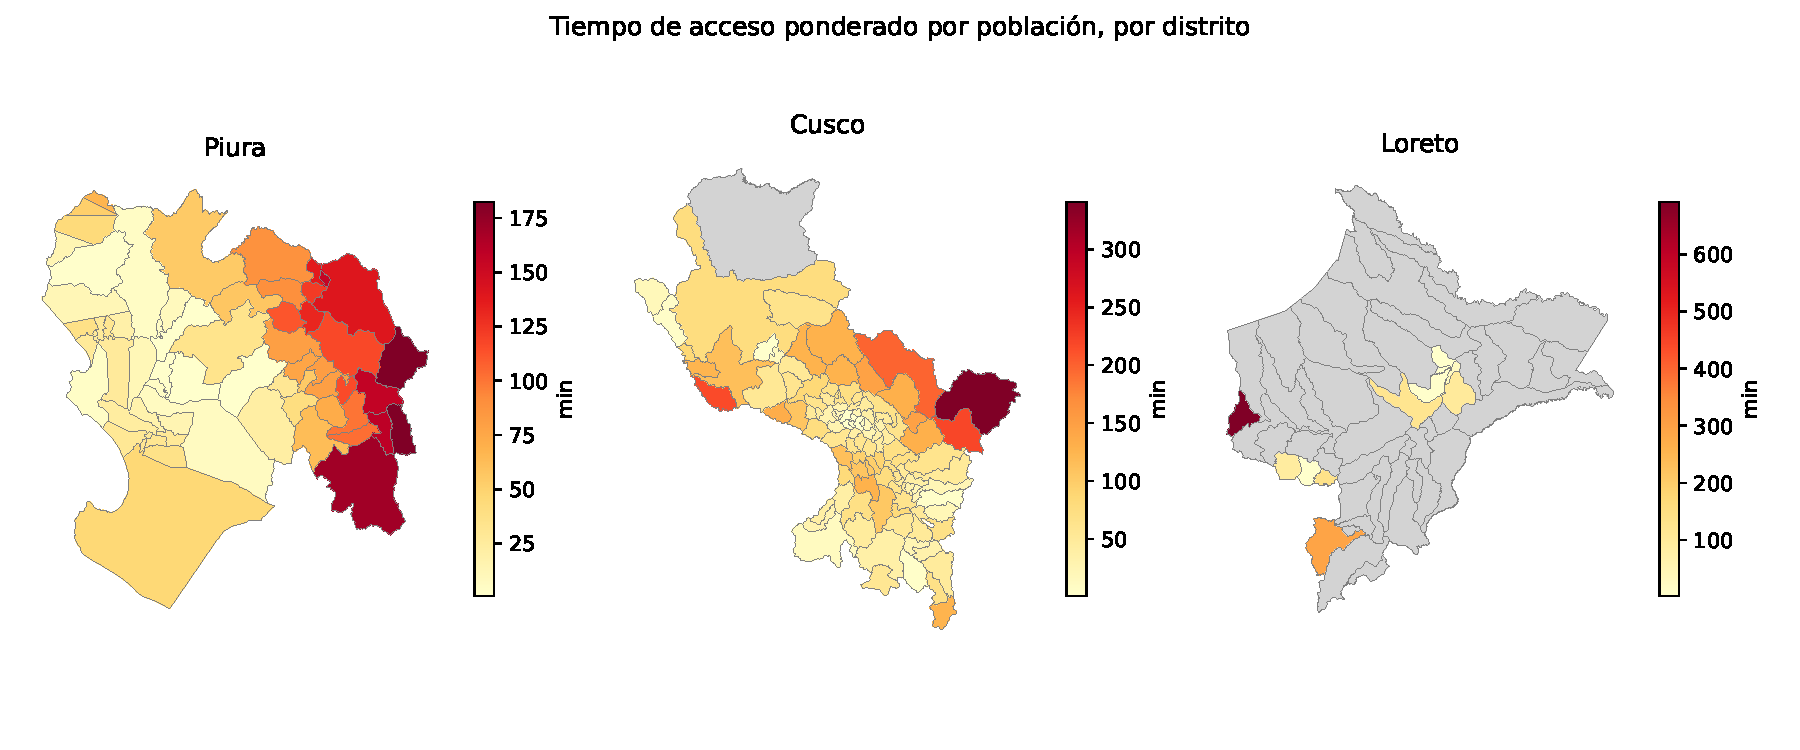
\includegraphics[width=\textwidth]{figures/mapa_distrital.pdf}
  \caption{Tiempo de acceso ponderado por distrito.}
  \label{fig:mapa}
\end{figure}

\subsection{Cruce con tama\~no de poblaci\'on}

Se explor\'o la relaci\'on entre el tama\~no poblacional del centro
poblado y su tiempo de acceso, como proxy de ruralidad/aislamiento. La
correlaci\'on de Spearman es d\'ebil en los tres departamentos por
separado (entre $-0.12$ y $0.06$, verificado que no es un efecto Simpson
por agregaci\'on): el tama\~no del asentamiento no predice bien el tiempo
de acceso en estos datos. De existir, la relaci\'on ser\'ia correlacional
y no causal: es plausible que la causalidad vaya en ambos sentidos, ya
que los establecimientos y las v\'ias tienden a ubicarse donde ya hay
poblaci\'on concentrada.

\section{Discusi\'on: distancia recta vs. distancia por red}

El enunciado pide comparar, para cada punto de demanda, el establecimiento
resolutivo m\'as cercano en l\'inea recta contra el m\'as r\'apido por
carretera. Los resultados (Figura~\ref{fig:ecdf}) muestran una discrepancia
sustancial: el establecimiento coincide en solo 50.3\% de los puntos en
Piura y 75.2\% en Cusco, con un factor de desv\'io promedio (distancia por
red / distancia recta) de 1.87x y 1.90x respectivamente. En Loreto, sobre
el subconjunto routeable, la coincidencia es 55.7\% pero el factor de
desv\'io es menor (1.18x) porque la escasa red vial obliga a rutas casi
rectil\'ineas donde existen, aunque muchas veces esas rutas no llegan a
ning\'un lado \'util.

\begin{figure}[H]
  \centering
  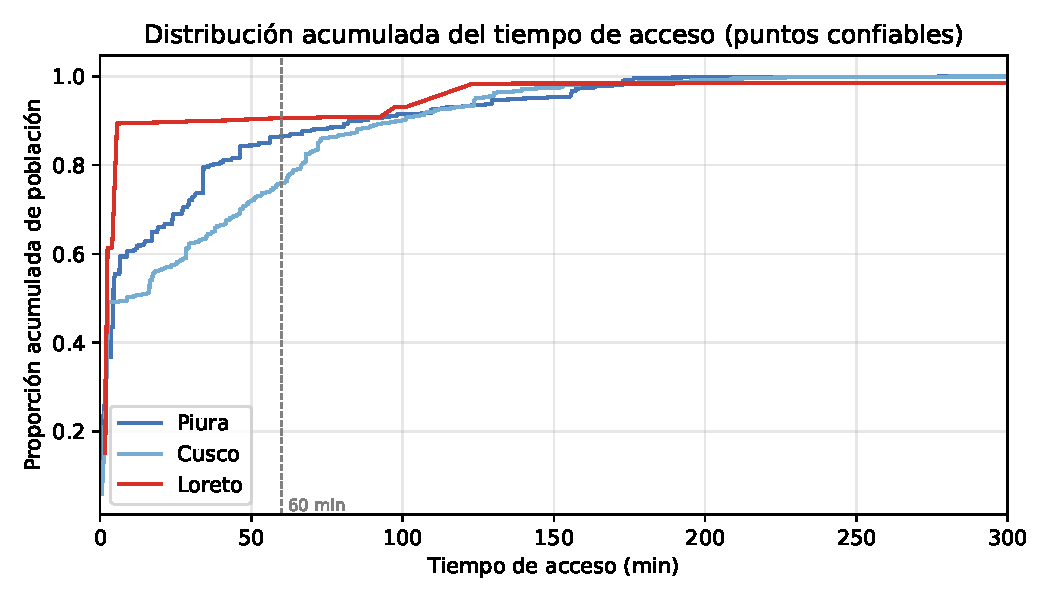
\includegraphics[width=0.85\textwidth]{figures/ecdf_acceso.pdf}
  \caption{Distribuci\'on acumulada del tiempo de acceso por
  departamento (solo puntos confiables).}
  \label{fig:ecdf}
\end{figure}

Esta discrepancia no es un defecto del pipeline: es exactamente el tipo
de sesgo que un an\'alisis basado en distancia eucl\'idea introducir\'ia
si se usara en lugar de ruteo real. Es mayor en zonas donde la topograf\'ia
o la disposici\'on de las v\'ias obliga a rodeos significativos ---la
sierra de Piura y los valles cusque\~nos, donde una l\'inea recta a menudo
cruza monta\~nas sin v\'ias--- y menor en la selva baja, donde no hay
suficiente red vial para que un rodeo sea siquiera posible.

\section{Limitaciones}
\label{sec:limitaciones}

\begin{itemize}
  \item \textbf{Cobertura de OpenStreetMap en la Amazon\'ia.} Este es el
  l\'imite metodol\'ogico central del proyecto, no una nota al pie. La
  mediana de distancia de un punto de demanda de Loreto a la v\'ia mapeada
  m\'as cercana es 43.3\,km (percentil 99: 331\,km, m\'aximo 414\,km).
  86.2\% de los puntos de demanda de Loreto no cumplen el chequeo de
  confiabilidad, y 162 (9\%) no tienen ninguna ruta v\'alida a ninguna
  facility por estar en un componente de red desconectado. El an\'alisis
  de ``golden hour'' basado en ruteo vehicular es estructuralmente
  inadecuado para representar c\'omo se moviliza la mayor parte de la
  poblaci\'on amaz\'onica, que depende de transporte fluvial. Un motor de
  ruteo fluvial o multimodal para la selva queda fuera del alcance de
  este proyecto, pero es la extensi\'on obviamente necesaria para un
  an\'alisis v\'alido de Loreto.
  \item \textbf{Tasa de error de coordenadas en RENIPRESS.} 29\% de los
  establecimientos de los tres departamentos no tienen coordenadas
  utilizables, y 15.6\% de los geocodificados caen fuera de su distrito
  declarado (aunque dentro de un distrito real y contiguo, ver
  Secci\'on~4.2).
  \item \textbf{Supuesto de disponibilidad.} Se asume que un
  establecimiento listado como \texttt{ACTIVO} en RENIPRESS est\'a
  efectivamente operando y con personal, sin considerar disponibilidad de
  camas, quir\'ofano libre, o personal de guardia en el momento de la
  emergencia. RENIPRESS es un registro administrativo, no un sistema de
  disponibilidad en tiempo real.
  \item \textbf{Ausencia de disponibilidad de ambulancias.} El modelo
  asume que el paciente (o quien lo transporta) tiene acceso inmediato a
  un veh\'iculo; no se modela el tiempo de despacho de una ambulancia ni
  su disponibilidad real en zonas rurales.
  \item \textbf{Poblaci\'on urbana estimada, no censada directamente.} No
  existe una capa p\'ublica del geoportal IDEP con la poblaci\'on urbana
  concentrada como puntos individuales (todas las que se probaron cubren
  \'unicamente poblaci\'on ``dispersa''/rural). Se estim\'o
  $\text{poblaci\'on urbana} = \text{poblaci\'on total proyectada 2026} -
  \text{poblaci\'on dispersa censada}$, agregada en un \'unico punto por
  distrito (la capital distrital). Es una simplificaci\'on deliberada:
  razonable porque el inter\'es del an\'alisis es el tiempo de viaje hacia
  la ciudad, no la variaci\'on intraurbana, pero pierde granularidad
  dentro de las ciudades grandes.
  \item \textbf{Discrepancia residual de poblaci\'on.} La suma de la
  poblaci\'on distrital procesada no calza exactamente con la fila
  departamental del Excel de INEI: en Cusco falta 17{,}943 habitantes
  porque el Excel 2026 incluye 4 distritos creados en 2021 (Ley
  N.\textdegree\ 31197) que a\'un no existen en la capa de l\'imites
  administrativos usada (vigente a 2020); en Loreto falta 3{,}179
  habitantes, pero esa discrepancia ya exist\'ia dentro del propio
  Excel de INEI (la suma de sus filas distritales no iguala su fila
  departamental).
  \item \textbf{Vigencia de las fuentes.} Los l\'imites administrativos
  est\'an vigentes al 2020-07-14 y RENIPRESS al 31 de agosto de 2026;
  los datos censales de poblaci\'on dispersa provienen del Censo 2017,
  ajustados con proyecciones a 2026 solo para el agregado distrital, no
  por centro poblado individual.
  \item \textbf{Problemas de encoding detectados en las fuentes.} El
  campo \texttt{adm0\_name} de la capa de l\'imites administrativos
  contiene ``Per\'u'' corrompido a ``Per'' seguido del car\'acter de
  reemplazo Unicode U+FFFD (p\'erdida de byte),
  documentado como hallazgo de la regla de validaci\'on de encoding,
  aunque no afect\'o a RENIPRESS para estos tres departamentos.
  \item \textbf{Alcance geogr\'afico.} Los resultados de Piura, Cusco y
  Loreto no son necesariamente generalizables a otros departamentos con
  perfiles geogr\'aficos distintos.
\end{itemize}

\section{Conclusiones y recomendaciones}

El acceso vial a salud resolutiva en Per\'u no es un problema homog\'eneo:
es, ante todo, un problema de \emph{qu\'e tan bien mapeada est\'a la red
vial}, adem\'as de un problema de d\'onde est\'an los establecimientos. En
Piura y Cusco, donde la red de OpenStreetMap est\'a razonablemente
completa, el hallazgo dominante es que la distancia eucl\'idea subestima
sistem\'aticamente el tiempo real de viaje (factor de desv\'io ${\sim}1.9$x)
y que casi la mitad de la poblaci\'on tiene su facility resolutiva
geogr\'aficamente m\'as cercana equivocada si se usa esa aproximaci\'on. En
Loreto, el problema es anterior a cualquier c\'alculo de tiempo: no hay
suficiente red vial mapeada para que el concepto mismo de ``tiempo de
viaje en auto'' sea aplicable a la mayor\'ia de su poblaci\'on.

Se recomienda: (1) para Piura y Cusco, usar los resultados de este
an\'alisis para priorizar inversi\'on vial y ubicaci\'on de nuevos
establecimientos en los distritos cr\'iticos identificados (Tabla
\ref{tab:distritos_criticos}), apoy\'andose en el simulador de escenarios
del dashboard; (2) para Loreto, no usar este an\'alisis como base \'unica
de pol\'itica ---se requiere una fuente de datos de transporte fluvial
antes de que cualquier m\'etrica de ``tiempo de acceso'' sea confiable--- y
tratar el 43.9\% sin dato confiable expl\'icitamente como poblaci\'on cuya
accesibilidad real se desconoce, no como poblaci\'on sin problema; (3)
como extensi\'on de innovaci\'on natural de este proyecto: un modelo 2SFCA
que incorpore capacidad de los establecimientos (no solo distancia),
an\'alisis de sitios \'optimos para nuevos establecimientos resolutivos, y
un motor de ruteo multimodal (v\'ia + r\'io) para la Amazon\'ia.

\begin{thebibliography}{9}

\bibitem{renipress}
SUSALUD. \emph{Registro Nacional de Instituciones Prestadoras de Servicios
de Salud (RENIPRESS)}. Plataforma Nacional de Datos Abiertos del Per\'u.
\url{https://www.datosabiertos.gob.pe/dataset/registro-nacional-de-entidades-prestadoras-de-servicios-de-salud-renipress}

\bibitem{inei2017}
Instituto Nacional de Estad\'istica e Inform\'atica (INEI). \emph{Censos
Nacionales 2017: XII de Poblaci\'on, VII de Vivienda y III de Comunidades
Ind\'igenas --- Directorio Nacional de Centros Poblados}.

\bibitem{inei_proy}
Instituto Nacional de Estad\'istica e Inform\'atica (INEI). \emph{Per\'u:
Poblaci\'on Total Proyectada al 30 de Junio de cada A\~no, seg\'un
Departamento, Provincia y Distrito, 2018--2026}.

\bibitem{ign}
Instituto Geogr\'afico Nacional del Per\'u (IGN). Geoportal IDEP
(Infraestructura de Datos Espaciales del Per\'u).
\url{https://www.idep.gob.pe/geoportal/}

\bibitem{hdx}
OCHA Field Information Services Section. \emph{Peru --- Subnational
Administrative Boundaries (COD-AB)}. Humanitarian Data Exchange.
\url{https://data.humdata.org/dataset/cod-ab-per}

\bibitem{osm}
OpenStreetMap contributors. \emph{Extracto de Per\'u}. Geofabrik.
\url{https://download.geofabrik.de/south-america/peru.html}

\bibitem{osrm}
Luxen, D., Vetter, C. (2011). \emph{Real-time routing with OpenStreetMap
data}. Project OSRM. \url{http://project-osrm.org}

\bibitem{gini}
Gastwirth, J. L. (1972). The estimation of the Lorenz curve and Gini
index. \emph{The Review of Economics and Statistics}, 54(3), 306--316.

\end{thebibliography}

\end{document}
